\documentclass[11pt,letterpaper]{article}
\usepackage[margin=1in]{geometry}
\usepackage[T1]{fontenc}
\usepackage{lmodern,microtype,amsmath,amssymb,amsthm,mathtools}
\usepackage{booktabs,array,longtable,enumitem,listings,tikz}
\usepackage[hidelinks]{hyperref}
\hypersetup{pdftitle={Beyond Length Descent: Certified Whitehead Exposure for Unknot Recognition},
 pdfauthor={ProveIt research continuation},
 pdfsubject={Unit bridges, exact constrained cut optimization, and bounded positive-certificate search},
 pdfkeywords={unknot recognition, Whitehead automorphisms, minimum cuts, straight-line programs}}
\usepackage{fancyhdr}
\pagestyle{fancy}\fancyhf{}\fancyhead[L]{\small Certified Whitehead exposure}\fancyhead[R]{\small ProveIt research continuation}\fancyfoot[C]{\thepage}
\setlength{\headheight}{14pt}
\setlength{\parskip}{3pt}
\setlength{\emergencystretch}{2em}
\setlist{itemsep=3pt,topsep=4pt}
\lstset{basicstyle=\ttfamily\small,breaklines=true,columns=fullflexible,keepspaces=true,frame=single}
\newtheorem{theorem}{Theorem}[section]
\newtheorem{lemma}[theorem]{Lemma}
\newtheorem{proposition}[theorem]{Proposition}
\newtheorem{corollary}[theorem]{Corollary}
\theoremstyle{definition}\newtheorem{definition}[theorem]{Definition}
\newtheorem{example}[theorem]{Example}
\newtheorem{remark}[theorem]{Remark}
\newcommand{\cyc}{\operatorname{cycred}}
\newcommand{\fr}{\operatorname{fred}}
\newcommand{\capc}{\operatorname{cap}}
\newcommand{\occ}{\operatorname{occ}}
\newcommand{\Z}{\mathbb Z}
\newcommand{\set}[1]{\{#1\}}
\newcommand{\bits}{\operatorname{bits}}
\newcommand{\wh}{\varphi_{a,S}}
\newcommand{\repo}{\texttt{Topology/UnknotRecognition}}
\title{\textbf{Beyond Length Descent:}\\[3pt]
Certified Whitehead Exposure\\for Unknot Recognition\\[7pt]
\large Unit bridges, optimal elimination bounds,\\and a compressed obstruction family}
\author{ProveIt research continuation\\\small Prepared with AI assistance for mathematical review and integration}
\date{8 October 2026}
\begin{document}
\maketitle
\begin{abstract}
We develop an exact, polynomial-time local oracle for a positive-certificate branch of unknot recognition. Rather than minimizing total relator length, it seeks one Whitehead automorphism that makes a generator occur exactly once in a relation, enabling immediate Tietze elimination. A cyclic occurrence identity characterizes such exposure by a unit-weight bridge of the relation's Whitehead graph. Contracting all other edges reduces the constrained optimization to pinned minimum cuts, with substantial sharing between multipliers. The same cuts minimize an exact pre-cancellation allocation bound for the subsequent elimination.

An explicit family $P_m\cong\Z$ shows why this objective is genuinely different from length descent: for $m\ge2$, every non-inner elementary Whitehead move increases total length, yet one exposing move and one elimination finish. The smallest one-step exposing increase is $2m-2$. For $m=2^k$, exact selection and fused quotient replay use $k+51$ grammar nodes, without expanding the relators. A rank-first schedule has at most $r-1$ rank drops and a quasipolynomial-bounded implementation under an explicit length cap. It remains a one-sided search, not a complete general quasipolynomial recognizer.

The package supplies proofs, a standard-library implementation, separate replay checks, 49 unit tests, 17,664 exhaustive word/move checks, 640 selector comparisons against literal enumeration, and reproducible experiments. It also records negative evidence: no coverage gain on the supplied elementary braid corpus, and failure of the new stage to finish the 141-crossing Gordian fixture. Integration is opt-in; no production defaults are changed.
\end{abstract}
\vspace{3pt}
\noindent\textbf{Keywords.} Unknot recognition; Wirtinger presentations; Whitehead automorphisms; minimum cuts; straight-line programs; proof-carrying computation.
\newpage
\tableofcontents
\newpage

\section{Research objective and audited starting point}\label{sec:scope}
The goal of this continuation is to remove a specific restriction in the group-certificate branch of the ProveIt unknot recognizer: a useful automorphism need not shorten the current presentation if it immediately exposes a generator that can be eliminated. We give a complete local search for this event, account for its cost, and separate it from the global question of how often such events suffice on knot inputs.

The source audit is pinned to repository commit
\begin{center}\small\texttt{04d799b69d388f75ce85539b26fca1585f9d2651}.\end{center}
The relevant maintained files are \path{fast/fastunknot/group_certificate.py}, \path{fast/fastunknot/diagram.py}, and \texttt{fast/README.md} under \repo\ \cite{repo}. The group search already computes Whitehead moves by integer minimum cuts; it does \emph{not} enumerate all signed subsets. It first looks for a generator with one occurrence in some relation, uses a strict total-length decrease for ordinary Whitehead search, and optionally interleaves relator-overlap substitutions. Its independent certificate verifier already accepts valid Whitehead moves regardless of whether they shorten. Thus our proposal requires a new search objective, not a new topological inference rule or a new elementary certificate format.

The current repository contains compressed word kernels, Whitehead powers, relator powers, braid kernels, and several exact homological acceleration mechanisms. We do not repackage those results here. In particular, replacing exponential subset enumeration by ordinary minimum cut is classical \cite{rvw} and is already implemented upstream. The contribution is the \emph{singleton-constrained} problem, its post-elimination objective, its proof-oriented implementation, and the explicit obstruction to relying on non-increasing length alone.

The distinction from compressed primitivity is also important. A recent preprint of Kapovich treats compressed primitivity and compressed Whitehead minimality \cite{kapovich}. Our local query neither decides primitivity in general nor computes an automorphically shortest representative. It works in variable rank, exploits a particularly rigid target condition, and can deliberately choose a length-increasing move in a tuple of relators.

The wider complexity target must be described precisely. Lackenby's July 2026 hierarchy preprint gives a new algorithmic framework; its Section 9 explicitly separates counting steps from bounding their running time \cite{lackenby}. This article does not implement that hierarchy. It improves a different, exact positive-certificate branch and identifies an additional structural condition that would be needed to turn that branch into a complete quasipolynomial algorithm.

\subsection{What is established here}
Our principal statements are unconditional local theorems: the occurrence-cut identity, the unit-bridge characterization, a polynomial selector for all one-step exposures, the exact allocation formula, and the infinite family separating exposure from non-increasing descent. A bounded rank-first stage then gives an unconditional \emph{runtime bound for a possibly inconclusive search}. This distinction is not a technical footnote: a time-limited search is not a recognition algorithm unless it is proved to finish conclusively on every valid input.

The mathematical contribution is presented for scrutiny rather than as a claim of established historical priority. The unit-bridge criterion is an elementary but useful consequence of classical Whitehead theory. The combined optimization, explicit barrier family, and integration analysis are the focus of this continuation. No proof-assistant formalization or external peer review is claimed.

\section{Presentations, certificates, and notation}\label{sec:notation}
Let $F(X)$ be the free group with basis $X=\set{x_1,\ldots,x_r}$ and signed alphabet
$V=X\sqcup X^{-1}$. In implementations the signed letter $\pm i$ denotes $x_i^{\pm1}$. A presentation is a tuple
\[
 P=\langle X\mid w_1,\ldots,w_m\rangle,
\]
where every $w_j$ is freely and cyclically reduced. Empty relators are allowed and their indices are retained. Write $\ell_j=|w_j|$ and $L=\sum_j\ell_j$. A relation is \emph{defining for $g$} if its cyclic spelling contains exactly one occurrence of $g$ or $g^{-1}$.

The allowed elementary moves are simultaneous free-group automorphisms on all relators, cyclic reduction or cyclic conjugation of individual relators, and elimination of a generator using a defining relation. All are presentation isomorphisms or standard Tietze transformations. In particular, we never delete a nonempty relation merely because its abelianization vanishes.

\begin{proposition}[Positive topological conclusion]\label{prop:topology}
Suppose a classical one-component knot diagram in $S^3$ has been validated, its full Wirtinger presentation has been constructed, and a replayed sequence of the preceding moves ends with one generator and no nonempty relators. Then the diagram represents the unknot.
\end{proposition}
\begin{proof}
The replay proves that the knot group is the free group of rank one, hence isomorphic to $\Z$. A knot in $S^3$ is unknotted if and only if its group is free cyclic; this is the classical theorem recorded by Papakyriakopoulos \cite[Theorem 3(i)]{papa}. Validation and reconstruction bind the algebraic argument to the given diagram. A free-rank-one result for an arbitrary JSON presentation, without that binding, does not prove anything about an independently supplied diagram.
\end{proof}

The proposition is used only in the positive direction. Failure to expose a generator, exhaustion of a budget, or arrival at an ordinary Whitehead minimum is always inconclusive.

\subsection{The graph convention}
For a cyclic word $w$, let $G_w$ be the weighted undirected graph on $V$ obtained by adding one unit to the edge $\set{x,y^{-1}}$ for every cyclic consecutive pair $xy$ in $w$. Parallel edges are stored as one positive integer capacity. A reduced cyclic word gives no loops. A one-letter word $a$ gives the edge $\set{a,a^{-1}}$ of weight one; the empty word gives the empty graph.

Set $G_j=G_{w_j}$ and $G=\sum_jG_j$. For a shore $S\subseteq V$, define
\[
 c_j(S)=\capc_{G_j}(S),\qquad c(S)=\capc_G(S),
\]
where a cut capacity sums weights of edges with exactly one endpoint in $S$. Put $d_j(a)=\deg_{G_j}(a)$ and $d(a)=\deg_G(a)$.
\begin{lemma}[Signed degree balance]\label{lem:degree}
For every signed letter $a$, $d_j(a)=d_j(a^{-1})$ equals the number of occurrences of $a$ or $a^{-1}$ in $w_j$. Also $\sum_eG_j(e)=\ell_j$.
\end{lemma}
\begin{proof}
An occurrence of $a$ contributes once at the first endpoint of its outgoing cyclic pair, and an occurrence of $a^{-1}$ contributes once at the second endpoint of its incoming pair. These are exactly the incidences at $a$. The same count applies at $a^{-1}$. Every cyclic adjacent pair contributes one unit of edge weight, and there are $\ell_j$ such pairs.
\end{proof}

\subsection{Whitehead moves}
A characteristic pair $(a,S)$ is admissible when $a\in S$ and $a^{-1}\notin S$. The corresponding type-II Whitehead automorphism is
\begin{equation}\label{eq:whitehead}
 \wh(x)=a^{-\mathbf1_{x^{-1}\in S}}\,x\,a^{\mathbf1_{x\in S}}
 \quad (x\notin\set{a,a^{-1}}),\qquad \wh(a^{\pm1})=a^{\pm1}.
\end{equation}
This convention agrees with the audited upstream image rule. A signed permutation of the basis is called a type-I move. Every image of a single letter under \eqref{eq:whitehead} has length at most three. The literal total substitution workspace is consequently bounded by $3L$ before free reduction.

\section{An occurrence identity stronger than the length formula}\label{sec:occurrence}
The classical length formula is usually used to find a shortening cut. For exposure it is more informative to retain the individual occurrence count from which that formula follows.

\begin{theorem}[Occurrence-cut identity]\label{thm:occurrence}
Let $w$ be a cyclically reduced word and let $(a,S)$ be admissible. In $z=\cyc(\wh(w))$, the number of occurrences of $a$ or $a^{-1}$ is exactly $\capc_{G_w}(S)$. For each $g$ with $\set{g,g^{-1}}\ne\set{a,a^{-1}}$, the number of occurrences of $g$ or $g^{-1}$ is unchanged. Thus
\begin{equation}\label{eq:length}
 |z|-|w|=\capc_{G_w}(S)-\deg_{G_w}(a).
\end{equation}
\end{theorem}
\begin{proof}
The empty word is immediate. If $w$ contains only $a^{\pm1}$, cyclic reducedness makes it a pure signed power. The automorphism fixes it, while every graph edge is $\set{a,a^{-1}}$, which crosses the cut. Suppose now that $w$ contains a different signed letter. Up to cyclic rotation, write
\[
 w=b_1a^{e_1}b_2a^{e_2}\cdots b_qa^{e_q},\qquad b_i\notin\set{a,a^{-1}},
\]
with subscripts interpreted cyclically. The $b_i$ are single signed letters and some $e_i$ may be zero. Define $\chi(x)=\mathbf1_{x\in S}$. Substitution changes the exponent in the $i$th gap to
\begin{equation}\label{eq:gap}
 e_i'=e_i+\chi(b_i)-\chi(b_{i+1}^{-1}).
\end{equation}
If consecutive non-multiplier letters are inverse, $b_{i+1}=b_i^{-1}$, their two indicators in \eqref{eq:gap} agree. The original exponent $e_i$ is nonzero, because $w$ is reduced, and therefore $e_i'$ is nonzero too. No inverse pair among the $b_i$ can cancel. After reducing each multiplier gap, the entire cyclic word is reduced: any remaining possible cancellation would have to be between such an inverse pair separated by a zero gap, which was just excluded. This proves invariance of all non-multiplier counts, including at the cyclic seam.

It remains to identify $\sum_i|e_i'|$ with the cut capacity. Partition the cyclic adjacent pairs into the paths from $b_i$ to $b_{i+1}$ through the $i$th multiplier gap. If $e_i=0$, its single graph edge contributes
\[
 |\chi(b_i)-\chi(b_{i+1}^{-1})|=|e_i'|.
\]
If $e_i>0$, the first edge joins $b_i$ to $a^{-1}$ and contributes $\chi(b_i)$; the $e_i-1$ internal multiplier pairs each cross; and the final edge from $a$ to $b_{i+1}^{-1}$ contributes $1-\chi(b_{i+1}^{-1})$. Their sum is
\[
 e_i+\chi(b_i)-\chi(b_{i+1}^{-1})=e_i'=|e_i'|,
\]
since $e_i'\ge0$. If $e_i<0$, the analogous sum is
$-e_i-\chi(b_i)+\chi(b_{i+1}^{-1})=-e_i'=|e_i'|$.
These paths partition all cyclic pairs, proving the count identity. Subtracting the original multiplier count gives \eqref{eq:length}.
\end{proof}

\begin{corollary}[Exact exposure constraint]\label{cor:exposure}
The multiplier of $(a,S)$ becomes defining in relation $j$ if and only if $c_j(S)=1$.
\end{corollary}
The equation is an equality of nonnegative integers, not a relaxation. In particular, minimizing the total cut $c(S)$ without imposing $c_j(S)=1$ need not locate a defining relation, even when a one-step exposure exists.

\section{The unit-bridge characterization}\label{sec:bridge}
A \emph{unit bridge} of a weighted graph means an edge of capacity one that is a bridge in the graph of positive-capacity edges. An edge of capacity two is not a unit bridge, even if its aggregated support edge is a graph-theoretic bridge.

\begin{theorem}[One-step singleton exposure]\label{thm:bridge}
For a cyclically reduced word $w$, the following are equivalent:
\begin{enumerate}[label=(\roman*)]
\item Some admissible type-II Whitehead move has a multiplier occurring exactly once in its cyclically reduced image of $w$.
\item There is a cut of $G_w$ of capacity one.
\item $G_w$ has a unit bridge.
\end{enumerate}
The equivalence includes words already having a singleton; identity characteristic pairs are allowed. If all current relations lack a singleton, every successful witness creates one that was not previously available.
\end{theorem}
\begin{proof}
The implication (i)$\Rightarrow$(ii) is Corollary~\ref{cor:exposure}. A capacity-one cut has exactly one crossing support edge, and that edge has weight one. Any alternate support path between its endpoints would cross the cut again. Therefore the edge is a bridge, proving (ii)$\Rightarrow$(iii).

For (iii)$\Rightarrow$(i), delete a unit bridge $e$ and choose $S$ to be the vertices of one of the two components into which its original support component splits. Put every other support component outside $S$. Then $\capc_{G_w}(S)=1$. The weighted degree sum over $S$ is twice the internal edge weight plus one, hence odd. If $S$ were invariant under inversion, Lemma~\ref{lem:degree} would make that degree sum even. Thus $S$ separates an inverse pair. Choose $a\in S$ with $a^{-1}\notin S$. It is an admissible multiplier, and Theorem~\ref{thm:occurrence} gives a singleton.
\end{proof}

\subsection{Detection cost and absent letters}
An iterative depth-first search finds all support bridges using discovery times and low-link values. It runs in $O(r+|E(G_w)|)$ graph operations and avoids recursive call-stack dependence. The capacity test then discards every bridge of weight greater than one. The signed alphabet must include absent letters: they are isolated vertices and will matter in the optimization on the \emph{other} relators. Omitting them is harmless for detecting existence in a single word, but can make the tuple optimizer incomplete.

\begin{figure}[ht]
\centering
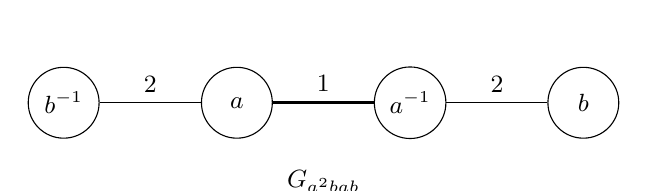
\begin{tikzpicture}[every node/.style={font=\small}]
\node[circle,draw,minimum size=9mm] (a) at (0,0) {$a$};
\node[circle,draw,minimum size=9mm] (B) at (-2.2,0) {$b^{-1}$};
\node[circle,draw,minimum size=9mm] (A) at (2.2,0) {$a^{-1}$};
\node[circle,draw,minimum size=9mm] (b) at (4.4,0) {$b$};
\draw (B)--node[above]{2}(a);
\draw[very thick] (a)--node[above]{1}(A);
\draw (A)--node[above]{2}(b);
\node at (1.1,-1.0) {$G_{a^2bab}$};
\end{tikzpicture}
\caption{The middle edge is the unique unit bridge. Its two shores force the exposing cut when the whole signed alphabet is $\set{a^{\pm1},b^{\pm1}}$.}
\label{fig:bridge}
\end{figure}

\section{Complete constrained optimization by contraction}\label{sec:selector}
Existence is easy once the local graph is known. The optimization problem is more demanding because all other relators are transformed simultaneously. We seek the best total cost among \emph{all} characteristic pairs exposing \emph{any} relation, not just the cut obtained by deleting a bridge and arbitrarily assigning disconnected components.

Fix a relation $j$ and a unit bridge $e=\set{u,v}$ of $G_j$. Contract every support edge of $G_j-e$. Let $Q$ be the quotient vertex set, let $\pi:V\to Q$ be the component map, and push forward the total weighted graph $G$ to a graph $H$ on $Q$, discarding edges whose endpoints coalesce. In particular, capacities from every relation contribute to $H$.

\begin{lemma}[Cut correspondence]\label{lem:quotient}
The cuts $S\subseteq V$ whose sole crossing edge in $G_j$ is $e$ are exactly the inverse images of quotient shores $T\subseteq Q$ separating $\pi(u)$ and $\pi(v)$. For such shores,
$\capc_G(S)=\capc_H(T)$.
\end{lemma}
\begin{proof}
Every edge of $G_j-e$ must have both endpoints on the same side, so each of its components must be monochromatic. Conversely, a union of those components that separates the endpoints of $e$ crosses precisely $e$ locally. The total capacity identity follows by summing capacities on the quotient; discarded edges never cross.
\end{proof}

For a candidate multiplier $a$, require in addition that $\pi(a)$ be inside and $\pi(a^{-1})$ outside. We fix $\pi(u)$ inside and $\pi(v)$ outside, with $(u,v)$ chosen by the implementation's canonical signed ordering. A conflicting pin assignment is infeasible. Every other pin assignment is an ordinary minimum-cut problem with at most two inside and two outside pins.

\begin{lemma}[Complement symmetry]\label{lem:complement}
Replacing $(a,S)$ by $(a^{-1},V\setminus S)$ changes the automorphism only by a common inner conjugation. In particular it leaves every cyclic image length and every unsigned occurrence count unchanged.
\end{lemma}
\begin{proof}
For a non-multiplier letter $x$, direct substitution in \eqref{eq:whitehead} gives
\[
 \varphi_{a^{-1},V\setminus S}(x)=a\,\varphi_{a,S}(x)\,a^{-1}.
\]
The same equation holds on $a^{\pm1}$. Thus it holds on every word. Cyclic reduction preserves conjugacy-class length and the counts in a cyclic representative.
\end{proof}

It follows that fixing the orientation of the bridge loses no optimal value: a cut with the other orientation can be complemented while also inverting the multiplier. For each bridge, enumerate the signed multipliers. When $\pi(a)=\pi(a^{-1})$ discard the multiplier. Otherwise solve the pinned cut and score its capacity. Iterate over all unit bridges and all relations.

\begin{theorem}[Complete one-step selector]\label{thm:selector}
The preceding algorithm returns a one-step exposure whenever one exists. For each fixed target relation and multiplier it finds the least possible total cut capacity, up to the complement symmetry. Consequently it finds a globally minimum total Whitehead length change among all one-step exposures.
\end{theorem}
\begin{proof}
Any exposure has local cut capacity one. By Theorem~\ref{thm:bridge}, its unique crossing edge is a unit bridge. Lemma~\ref{lem:quotient} maps its shore to the quotient for that bridge. After complementing when necessary, the enumerated multiplier has precisely the required pin constraints. Minimum cut produces a feasible shore of no greater total capacity. Since $d(a)$ is fixed for a multiplier, \eqref{eq:length} shows that no larger total image length results. Conversely, every returned shore is admissible and has local capacity one, so it is a genuine exposure. Taking the minimum over the finite enumerated cases proves the claim.
\end{proof}

\subsection{Pattern sharing and the connected special case}
Two multipliers with the same ordered pair $(\pi(a),\pi(a^{-1}))$ induce the same pinned cut problem. Their degree terms and final scores may differ, but the optimal capacity can be cached. If $q=|Q|$, there are at most
\begin{equation}\label{eq:patterns}
 \min(2r,q(q-1))
\end{equation}
distinct nontrivial patterns. If the full local support graph $G_j$ is connected on all $2r$ signed vertices, then deleting a bridge yields $q=2$. Every feasible shore is forced; no maximum-flow call is necessary.

The condition ``on all signed vertices'' is essential. A relation using only $a,b$ in a presentation of rank ten has many isolated signed vertices. Assigning those vertices affects the other relators and may change the total optimum even though the bridge picture inside $\set{a^{\pm1},b^{\pm1}}$ is connected.

\subsection{Checkable pinned optima}
The implementation adds a super-source and super-sink and gives every pin edge capacity
\[
 I=1+\sum_{e\in E(H)}H(e).
\]
A feasible original cut costs at most $I-1$, so a minimum cut cannot violate a pin. A feasible integral flow with value equal to the returned cut proves optimality by weak duality. The supplied checker verifies edge capacities, flow conservation, the terminal value, and equality with the original quotient cut capacity; it does not run maximum flow again. Forced cuts are checked directly.

This certificate proves the optimum for the \emph{selected pinned problem}. It does not certify that the producer inspected every possible bridge or multiplier. Global optimality is a theorem about the selector, supported computationally by exhaustive differential checks. Topological soundness needs only the replayed automorphism and elimination, not global optimality.

\section{Optimizing the following Tietze elimination}\label{sec:allocation}
Minimizing total length immediately after a Whitehead move can still be the wrong objective. If a defining relation is to be used immediately, the more relevant quantity is how much material its substitution may create in the \emph{remaining} relations.

Fix an exposure $(j,a,S)$ and abbreviate
\[
 c=c(S),\qquad t=\ell_j-d_j(a).
\]
By Theorem~\ref{thm:occurrence}, the transformed target has length $t+1$, while the entire transformed tuple has $c$ occurrences of the multiplier. The defining relation solves $a$ or $a^{-1}$ as a word of length $t$ in the other generators.

\begin{theorem}[Exact allocation objective]\label{thm:allocation}
After cyclic reduction of all Whitehead images, delete the defining relation and substitute its solution into all other relators. The total number of letters before the final free reductions is exactly
\begin{equation}\label{eq:allocation}
 U(j,a,S)=L-d(a)+t(c-2).
\end{equation}
Therefore the final cyclically reduced tuple has total length at most $U$. For a fixed $j,a$, minimizing $c$ also minimizes $U$. The quotient selector consequently finds the globally minimum value of $U$ over all one-step exposures.
\end{theorem}
\begin{proof}
The transformed total length is $L+c-d(a)$. Removing the target removes $t+1$ letters. Each of the remaining $c-1$ multiplier occurrences is replaced by a word of length $t$, changing the raw size by $t-1$. Thus the exact raw size is
\[
 [L+c-d(a)]-(t+1)+(c-1)(t-1)=L-d(a)+t(c-2).
\]
Cancellations only reduce it. Since $t\ge0$, the expression is nondecreasing in $c$ when the target and multiplier are fixed. The completeness argument of Theorem~\ref{thm:selector} applies with this score. Complement symmetry preserves $t,d(a)$ and $c$, so fixing the orientation of each bridge is still legitimate.
\end{proof}

When $t=0$, the relation is a one-letter defining relation and elimination simply deletes all occurrences of the multiplier; $U=L-d(a)$ is independent of the cut. When $c=1$, the multiplier occurs only in the target, and the formula gives the length of the remaining non-multiplier letters after deleting that target. These cases need no special algebraic convention.

The implementation breaks ties in $U$ by total Whitehead length change, then by deterministic relation and multiplier order. It can also select by total length change as its primary objective. With an allocation cap $M$, it discards precisely the pinned optima with $U>M$. Because $U$ is monotone in $c$, no worse-capacity cut for the same case could make the allocation affordable. An optional upper bound on the Whitehead increase can be imposed at the same time.

\begin{remark}[What the objective does not optimize]\label{rem:notactual}
$U$ is not the final reduced size, and a minimum-$U$ exposure need not minimize the final reduced size. The graph records occurrences and adjacent pairs, not all long cancellation relationships. Section~\ref{sec:barrier} gives a particularly sharp warning: $U=34m$ while the actual final tuple is empty. The algorithm uses $U$ as a proved allocation bound, not as a prediction that those letters survive.
\end{remark}

\section{Bit complexity and compressed graph construction}\label{sec:complexity}
We use a conventional bit model with dense generator names $1,\ldots,r$. Tildes below hide logarithmic indexing factors; capacities are arbitrary-precision nonnegative integers. A binary straight-line program (SLP) has rules of the form empty, signed letter, or concatenation of two earlier nonterminals. Its roots specify the relators. Let $s$ be its number of rules. We require the root expansions to be freely and cyclically reduced; this is checked by the summaries described below, not assumed on untrusted input.

Let $B$ bound the bit lengths of all rule expansion lengths, the total root length $L$, and the indexing parameters, with a harmless additive constant. For a trimmed grammar every rule occurs below a root, so one can take
\[
 B=O\bigl(\log(L+2)+\log(s+m+r+2)\bigr).
\]
If unused rules are retained, their lengths must also be included in $B$. The supplied implementation processes them rather than silently assuming trimming.

\subsection{Exact cyclic adjacency summaries}
For a nonterminal $A$, store its expansion length, its first and last letters when nonempty, the count of each signed letter, the count of each \emph{linear} directed adjacent pair, and a flag for free reducedness. For a concatenation $A=BC$, add the two count tables and add one directed pair $(\operatorname{last}(B),\operatorname{first}(C))$ when both words are nonempty. The reducedness flag is the conjunction of the child flags and the condition that the join is not an inverse pair. At a root, check the cyclic seam and add its final-to-first pair to form the Whitehead graph.

\begin{proposition}[Compressed summary construction]\label{prop:slp}
The graphs of all roots can be constructed exactly without expansion in
\[
 \widetilde O(sr^2B+mr^2B)
\]
bit time and space. The root reducedness checks are exact. No algorithm for \emph{free-reducing an arbitrary compressed input} is asserted by this construction.
\end{proposition}
\begin{proof}
There are at most $2r$ signed-letter counts and $(2r)^2$ directed-pair counts per rule. A concatenation performs additions on $B$-bit integers and one possible seam increment. First and last letters are selected from the nonempty children. A concatenation is reduced exactly when both children are reduced and its single join has no cancellation; any internal failure remains a failure of the raw concatenation. The same observation checks the cyclic root seam. Mapping directed pairs to unordered Whitehead edges and adding the cyclic seam costs at most $O(r^2)$ count operations per root. Summing these bounds proves the claim.
\end{proof}

This summary construction is related to existing compressed Whitehead graph methods \cite{kapovich}; its purpose here is to make the input contract and the additional constrained optimization explicit. If a transformation produces an unreduced compressed word, an exact compressed reduction routine is still needed before applying this oracle again. Upstream already has such word infrastructure, but this standalone package does not duplicate it.

\subsection{A refined selector bound}
For each local graph let $c_j$ be its number of connected support components, counting every absent signed letter as an isolated component, and let $b_j$ be its number of unit bridges. Deleting a bridge increases the component count by one, so every bridge quotient for this relation has
\[
 q_j=c_j+1,\qquad b_j\le2r-c_j.
\]
The latter inequality follows because every bridge belongs to a spanning forest.

We use Edmonds--Karp for reproducibility, not because it is the fastest available flow method. Its breadth-first augmenting paths give $O(v e^2)$ arithmetic operations for a network with $v$ vertices and $e$ edges \cite{ek}; the bound is independent of the numerical value of the capacities. Here $v=O(q_j)$ and $e=O(q_j^2)$, so a call costs $\widetilde O(q_j^5B)$ bit operations. The pin capacities add only logarithmically many bits already absorbed into $B$.

\begin{theorem}[Polynomial local complexity]\label{thm:localcomplexity}
From the exact local graphs, the exposure selector can be implemented in
\begin{equation}\label{eq:refinedcost}
\widetilde O\!\left(mr^2B+
 \sum_{j=1}^{m} b_j\bigl[r^2B+rB^2+
 \min(r,q_j^2)q_j^5B\bigr]\right)
\end{equation}
bit time. Adding SLP summaries gives a conservative bound
\begin{equation}\label{eq:coarsecost}
 \widetilde O\bigl((s+m)r^2B+mr^7B+mr^2B^2\bigr).
\end{equation}
In particular, the local query is polynomial even when rank is part of the input and the relator lengths are exponential in the grammar size.
\end{theorem}
\begin{proof}
Bridge discovery and the local degree tables cost $\widetilde O(mr^2B)$ in a dense representation. For each bridge, contracting the local edges and pushing forward the total graph costs $\widetilde O(r^2B)$. At most $2r$ signed multipliers are scored. Computing the product in \eqref{eq:allocation} with schoolbook multiplication gives the conservative $\widetilde O(rB^2)$ term. By \eqref{eq:patterns}, the number of distinct pinned problems is $O(\min(r,q_j^2))$. Apply the preceding flow bound and sum. Finally $b_j=O(r)$ and $q_j=O(r)$ give \eqref{eq:coarsecost}, together with Proposition~\ref{prop:slp}.
\end{proof}

The bound is deliberately loose. For a connected local graph $q_j=2$, all feasible cuts are forced, so the flow term should be omitted rather than paid literally. Sparse graphs, reuse of the total graph, and incrementally maintained components can all improve constants. None of those optimizations is needed to establish polynomiality.

\subsection{Certificates and arithmetic magnitude}
The elementary Whitehead witness consists only of a multiplier and a signed subset. A local cut-optimality witness has at most $O(q_j^2)$ flow entries with $O(B)$ bits each, plus its shore. Large expanded lengths therefore create large integers, not a need to expand the words. Checking unsigned degree balance is a useful corruption test, but it does not establish that a supplied graph came from the asserted relator. The graph must be reconstructed from the actual word or grammar before any topological conclusion.

\section{A bounded rank-first positive-certificate stage}\label{sec:rankfirst}
Let $r_0,m_0$ be the initial presentation rank and number of relation slots. Fix a stored-letter allowance $M\ge L_0$. The following stage uses the exposed-generator objective as a bounded alternative to an unbounded sequence of length-improving moves.

At each iteration, first choose an already defining relation, when one exists, using its exact raw substitution bound. If this selected substitution exceeds $M$, stop inconclusively. If no defining relation is available, run the complete one-step exposure selector with the constraint $U\le M$. When it succeeds, apply its Whitehead move and immediately eliminate its multiplier. When it fails, stop inconclusively. If rank reaches one, return a positive certificate only when all relators are empty.

The rule for an unaffordable direct elimination is part of the implemented policy; it does not branch over arbitrary preparatory automorphisms. Likewise, the stage does not first perform all available strict Whitehead reductions. These design decisions make the rank-drop accounting transparent, but they mean that this stage should be interleaved with, or placed after a bounded probe of, the existing broader search rather than substituted for it globally.

\begin{theorem}[Rank-drop and certificate bounds]\label{thm:rankdrops}
Every nonterminal iteration of the rank-first stage decreases the number of active generators by exactly one. There are at most $r_0-1$ such iterations and at most $2(r_0-1)$ elementary moves. The literal Whitehead workspace is at most $3M$ and the stored tuple after every completed iteration has length at most $M$.

The standardized elementary certificate, excluding the original input, has
$O(r_0^2\log(r_0+m_0+2))$ bits. A positive result can be checked by an independent literal replay with the same order of workspace allowance.
\end{theorem}
\begin{proof}
A direct step eliminates one active generator. An exposure step is one automorphism followed by one valid elimination, also eliminating exactly one generator. Neither introduces generators. The loop stops at rank one or earlier. The workspace bound follows from the length-at-most-three letter images, while \eqref{eq:allocation} bounds each completed substitution by $M$. A Whitehead subset contains at most $2r_0$ signed indices, and each elimination names a relation and a generator. There are $O(r_0)$ moves of each kind, giving the certificate bound. Literal replay reconstructs the automorphism images, checks the defining occurrence, performs the substitution, and tests the terminal presentation; it needs no minimum-cut computation.
\end{proof}

For an explicit presentation, rebuilding graph summaries in every iteration is at worst linear in its expanded length times an integer-arithmetic factor. With
$B_0=1+\lceil\log_2(M+r_0+m_0+2)\rceil$, a convenient coarse implementation bound, including replay, is
\begin{equation}\label{eq:stagebound}
 \widetilde O\bigl(1+r_0MB_0+m_0r_0^8B_0^2\bigr).
\end{equation}
To see this, use the local graph bound with $r\le r_0$, pay for at most $r_0$ iterations, and include all literal substitution and replay work. The exponent is not an optimized claim about practical performance. It demonstrates that an unknown number of unit-length descents is not hidden in this particular schedule.

\begin{corollary}[Quasipolynomial-bounded search]\label{cor:qp}
For a validated $n$-crossing knot input with a linear-size initial Wirtinger presentation, choose
\[
 M(n)=\left\lceil\exp\bigl(C(\log(n+2))^d\bigr)\right\rceil,
 \qquad C>0,\quad d\ge1 \text{ fixed}.
\]
The rank-first stage, including its elementary replay, terminates in
$\exp(O((\log(n+2))^d))$ bit time. Every positive answer is sound. The statement does not assert that every unknot produces a positive answer.
\end{corollary}
\begin{proof}
The initial numbers of generators and relations are $O(n)$ and the initial letter count is $O(n)$; a crossingless knot is handled directly. Substitute these parameters and $B_0=O((\log(n+2))^d)$ into \eqref{eq:stagebound}. Soundness follows from Proposition~\ref{prop:topology} and the replay. Nothing in the complexity calculation proves that the selector succeeds at every iteration on every unknot.
\end{proof}

For $d=2$ this is of the familiar form $2^{O(\log^2 n)}$. Running a complete exact fallback after an inconclusive stage preserves correctness but not this general runtime bound: the fallback may still take exponential time. An existence theorem for \emph{some} short rank-dropping path would also not automatically prove success of this deterministic greedy policy. Either the path must be supplied with a bounded verifier, a controlled search must find it, or a theorem must guarantee the chosen policy's progress.

\section{An infinite obstruction to non-increasing length descent}\label{sec:barrier}
We now give a family that separates the new objective from a mere acceleration of old length descent. Let $F=F(a,b)$ and define
\begin{equation}\label{eq:family}
 u=a^2bab,\qquad t=(ab^{-1})^3,\qquad
 v=\cyc(utu^{-1}t^{-1}),\qquad
 P_m=\langle a,b\mid u,v^m\rangle \quad(m\ge1).
\end{equation}
Here $|u|=5$ and $|v|=20$. A convenient cyclic spelling of $v$, using uppercase letters for inverses, is
\[
 v=\texttt{ababaBaBaBBA BAA bAbAb}
\]
with spaces ignored; to remove any ambiguity, its exact signed encoding is
\begin{equation}\label{eq:vlist}
 (1,2,1,2,1,-2,1,-2,1,-2,-2,-1,-2,-1,-1,2,-1,2,-1,2).
\end{equation}
Only the signed encoding is used by the implementation.

\begin{theorem}[Presentation and descent barrier]\label{thm:barrier}
For every $m\ge1$, $P_m$ presents $\Z$ and has no defining relation in its displayed generators. A single Whitehead exposure followed by elimination proves this.

For $m=1$, no strictly length-decreasing type-II move exists, but a length-preserving exposure exists. For $m\ge2$, every non-inner type-II move increases total cyclic relator length. Any sequence of individually non-increasing type-I and type-II moves preserves the absence of a singleton. The smallest possible total increase of a \emph{single exposing} Whitehead move is exactly $2m-2$.
\end{theorem}
\begin{proof}
Let $\alpha(a)=a$ and $\alpha(b)=a^{-1}b$. This is \eqref{eq:whitehead} with multiplier $a$ and shore $\set{a,b^{-1}}$. Direct reduction gives
\[
 \alpha(u)=ab^2.
\]
Consequently $u$ is primitive: $ab^2$ extends to a free basis, and $\alpha$ is an automorphism. The second relator $v^m$ lies in the normal closure of $u$, since $v$ is conjugate to the commutator $[u,t]$. The first relation therefore gives $P_m\cong\langle a,b\mid u\rangle\cong\Z$. More constructively, apply $\alpha$, solve $a=b^{-2}$ from $ab^2=1$, and substitute. The image of $v^m$ becomes the identity, so no nonempty relator remains. Neither displayed relation initially has a singleton: $u$ contains three $a$ letters and two $b$ letters, while $v^m$ contains $10m$ occurrences of each generator up to sign.

For the exact descent calculation, the nonzero graph weights are as follows.
\begin{center}
\begin{tabular}{lrr}
\toprule Edge & $G_u$ & $G_v$\\\midrule
$\set{a,b^{-1}}$ & 2 & 4\\
$\set{a^{-1},b}$ & 2 & 4\\
$\set{a,a^{-1}}$ & 1 & 1\\
$\set{b,b^{-1}}$ & 0 & 1\\
$\set{a,b}$ & 0 & 5\\
$\set{a^{-1},b^{-1}}$ & 0 & 5\\\bottomrule
\end{tabular}
\end{center}
These counts can be obtained directly from \eqref{eq:vlist}; the weights sum to 5 and 20. The graph of $v^m$ is $mG_v$. There are 16 admissible characteristic pairs in rank two. Eight are identity or inner conjugation. The remaining eight occur in complement pairs, and their length changes on $(u,v)$ are
\begin{equation}\label{eq:slopes}
 (-2,2),\quad(-1,2),\quad(2,0),\quad(3,0).
\end{equation}
For transparency, a complete table is given in Appendix~\ref{app:movetable}; each entry follows from the four-vertex cut calculation in Theorem~\ref{thm:occurrence}. On $(u,v^m)$ the corresponding total changes are
\begin{equation}\label{eq:barrierdeltas}
 2m-2,\quad2m-1,\quad2,\quad3.
\end{equation}
Thus no strict decrease is available for $m\ge1$, and every non-inner move increases length for $m\ge2$.

For $m\ge2$, an individually non-increasing step is therefore inner or a signed permutation. Inner conjugation changes each cyclic representative only by cyclic rotation, and a signed permutation only relabels the graph and the occurrence counts. The same classification consequently applies after every such step, by induction, and no singleton appears.

Finally, $G_u$ has exactly one unit bridge, namely $\set{a,a^{-1}}$; $G_v$ has none, and multiplying all capacities by $m$ cannot create one. The two non-inner complement classes that expose $u$ have the first two slopes in \eqref{eq:slopes}. Their total increases are $2m-2$ and $2m-1$. Therefore $2m-2$ is the exact minimum for a single exposing move, including $m=1$.
\end{proof}

\subsection{Sharp cost accounting on the family}
For the first exposing class,
\[
 L=20m+5,\quad d(a)=10m+3,\quad c=12m+1,\quad t=2.
\]
It follows that
\begin{equation}\label{eq:familycost}
 L_{\mathrm{WH}}=22m+3,\qquad U=34m,\qquad L_{\mathrm{final}}=0.
\end{equation}
This is a structural separation, not a timed speedup between two successful implementations. The strict descent comparator stops inconclusively, whereas exposure finishes. Nor does the example show that the upstream overlap-enabled pipeline fails: a relator replacement can exploit the visible normal-closure dependence. The family isolates the automorphism-only descent restriction.

The lower bound $2m-2$ is about \emph{one-step exposure}. It is not a theorem that every longer path using increasing moves must have a peak of that height. It also is not yet a family of hard knot diagrams: the presentations are constructed algebraically and must not be counted as end-to-end knot benchmarks.

\section{Fused quotient replay on exponentially long relators}\label{sec:fused}
The bound $U$ is intentionally conservative. Constructing every intermediate word before eliminating the generator can be wasteful when the composite quotient map has small images. We therefore separate selecting an exposure from materializing its entire intermediate presentation.

Suppose the target image $z=\cyc(\wh(w_j))$ has a unique occurrence of $g^{\pm1}$, where $g$ is the positive generator underlying $a$. Solving the defining relation gives a word $R$ in the remaining generators. Let $q$ substitute $g\mapsto R$ and fix the others. Define the homomorphism
\[
 \psi=q\circ\wh:F(X)\longrightarrow F(X\setminus\set{g}).
\]
The remaining presentation is obtained by evaluating $\psi(w_i)$; constructing all of $\wh(w_i)$ first is unnecessary.

\begin{proposition}[Sound fused replay]\label{prop:fused}
A verifier may establish the target singleton, construct $\psi$ on the signed alphabet, and evaluate $\psi$ directly on every original relation. If all evaluated relators reduce to the identity, then the original presentation is a free group of rank $r-1$. In rank two this is a free-rank-one certificate.
\end{proposition}
\begin{proof}
The Whitehead move is an automorphism. Replacing the target relation by a cyclic conjugate does not change its normal closure. Because $g$ occurs exactly once, deleting that target and substituting its solved value is a valid Tietze elimination. Its other relators are precisely the free-group elements $q(\wh(w_i))=\psi(w_i)$. If they are all trivial, the resulting presentation has the remaining generators and no relations. Checking the target under $\psi$ as well is redundant mathematically but guards against accidental omission in code.
\end{proof}

\subsection{A bounded DAG-image evaluator}
The provided evaluator processes grammar rules in topological order. A terminal stores its image under $\psi$; a concatenation stores the freely reduced concatenation of its child images. It explicitly limits the literal reduction stack at every processed node. Exhaustion raises a resource exception, not a positive or negative verdict. This is a \emph{small-image evaluator}, not a general polynomial compressed word algorithm.

If every needed node has reduced image length at most $Q$ and every terminal image has length at most $Q$, a stack allowance $2Q$ suffices: each internal concatenation has at most $2Q$ letters before reduction. Evaluation then uses $\widetilde O(sQ\log(r+2))$ bit operations for the word part and $O(sQ\log(r+2))$ bits to store all images. Input-summary construction and target evaluation must be added. The meaningful parameter is the image size of \emph{all needed grammar nodes}, not merely the final root images; a root can be empty after cancellation even though an intermediate node has a huge image.

\begin{theorem}[Compressed barrier certificate]\label{thm:compressedbarrier}
For $m=2^k$, the family $P_m$ has a binary grammar with $k+51$ nodes. Exact graph construction, optimal exposure selection, local cut verification, and fused free-rank-one replay can all be carried out in $O((k+1)^2)$ bit time with no expansion to length $\Theta(2^k)$. A fixed literal-image stack cap of 100 suffices for the supplied grammar.
\end{theorem}
\begin{proof}
Build $u$ and the 20-letter $v$ by left-associated concatenations, using one empty node and two nodes per letter. This uses $1+2(5+20)=51$ nodes. Append $k$ squaring rules for $v$ and use the last as the second relation root. Every raw root is cyclically reduced. There are constantly many nonzero adjacency counts, with $O(k+1)$ bits, so the summaries use $O((k+1)^2)$ bit time. The selected target graph is connected on four vertices; its feasible bridge cuts are forced, and its score uses $O(k+1)$-bit integers.

Choose the exposing class of Theorem~\ref{thm:barrier}. For $\alpha(a)=a$, $\alpha(b)=a^{-1}b$ followed by $a=b^{-2}$, the composite map sends $a$ to $b^{-2}$ and $b$ to $b^3$. Signed images have length at most three. Every prefix node of the 20-letter base word has raw image length at most 60; the target image is smaller. The base word $v$ maps to the identity. Each subsequent squaring rule therefore concatenates two empty images. The complement-symmetric representative returned by the implementation has the same bounded quotient images. Thus cap 100 succeeds uniformly in $k$, and the word-evaluation part uses only linear work in the number of rules. Repeated exact summary validation and the integer arithmetic remain within $O((k+1)^2)$ bit time.
\end{proof}

The ordinary explicit rank-first stage with a small $M$ would reject this family's raw bound $U=34\cdot2^k$. The fused path is a separate exact way to avoid that allocation. A global compressed rank-first engine would additionally need bounded representation maintenance after every accepted quotient. Only the single-exposure fused verifier and the explicit iterative stage are implemented here.

\section{Precise limitations and further obstructions}\label{sec:limits}
The bridge criterion is complete for its stated local event, not for arbitrary primitive elements or arbitrary cyclic presentations. Several small examples prevent overgeneralization.

\subsection{A primitive word with no one-step exposure}
Consider
\[
 w=a^2ba^2bab.
\]
Its Whitehead support graph is a path with edge weights $3,2,3$, so it has no unit bridge. Therefore no single Whitehead move exposes a multiplier singleton. Nevertheless $w$ is primitive. First send $b\mapsto a^{-1}b$, obtaining the cyclic word $ababb$. Then send $a\mapsto b^{-1}a$, obtaining a cyclic conjugate of $a^2b$, which has a singleton $b$. Two further elementary shears send $a^2b$ to $b$. Each map is an automorphism, proving primitivity without an appeal to an external classifier.

Thus a ``no unit bridge'' response cannot be labeled nonprimitive. It is an exact negative answer to a \emph{one-step exposure query}. Even at rank two, an additional preparatory Whitehead move can change the answer.

\subsection{A cyclic presentation requiring relator interaction}
The presentation
\begin{equation}\label{eq:properpowers}
 \langle a,b\mid a^2,a^3\rangle
\end{equation}
is isomorphic to $\Z$, since $a^3(a^2)^{-1}=a$ lies in the normal closure of its relators. Yet neither relator can ever become defining under an automorphism alone. Indeed, an automorphism sends a nontrivial proper power to a proper power, and a cyclically reduced conjugate of $z^p$ repeats the cyclic core of $z$ exactly $p$ times. Every unsigned occurrence count is then a multiple of $p$, hence cannot be one when $p\ge2$.

This is a permanent obstruction to automorphism-only singleton exposure, not just a one-step obstruction. It explains why relator-overlap moves, Euclidean combinations of powers, or other justified relator replacements remain necessary. The existing repository already has mechanisms in this direction; exposure should cooperate with them.

\subsection{Simultaneous constraints are a different problem}
For one target relation, capacity one forces all but one local edge to stay uncut. After contraction, the admissibility condition is simply a few terminal pins. If several relations must simultaneously become defining, one must choose a unit bridge in each and make all corresponding parity constraints consistent. Contracting edges from several graphs can identify opposing pins or introduce coupled choices. The single-target minimum-cut theorem does not automatically imply an equally simple polynomial algorithm for the joint problem. We make no hardness claim here; an exact structural classification is a separate research task.

\subsection{Greedy progress is not guaranteed by an optimal local score}
The allocation objective controls one accepted move and its immediate elimination. It does not rank the future difficulty of the resulting presentations. Two equal-cost exposures can leave very different residual relators, and a more expensive exposure may make later reductions simpler. Consequently local optimality, a rank-drop bound, and a polynomial local oracle do not together prove global completeness. Our negative Gordian experiment in Section~\ref{sec:experiments} is an actual instance in which the implemented greedy path reaches a residual presentation with no local unit bridges.

\section{Implementation and verification architecture}\label{sec:implementation}
The companion package contains a standard-library Python implementation, tested here on CPython 3.13.5. Its main components are summarized below.
\begin{center}
\begin{tabular}{p{0.28\linewidth}p{0.65\linewidth}}
\toprule Module & Responsibility\\\midrule
\texttt{algebra.py} & Cyclic words, explicit Whitehead substitution, defining-relation elimination, exact weighted graphs, and local budgets.\\
\texttt{flow.py} & Deterministic pinned integer cuts and a separate flow/cut optimality checker.\\
\texttt{selector.py} & Unit bridges, quotient contraction, shared pin patterns, both score objectives, and exposure-witness checking.\\
\texttt{slp.py} & Exact raw-grammar summaries, bounded homomorphic-image evaluation, and fused quotient replay.\\
\texttt{engine.py} & Explicit rank-first search, a strict-descent comparator, and separate elementary presentation replay.\\
\texttt{braid.py} & A native classical braid-closure frontend and input-bound positive certificates for smoke experiments.\\
\texttt{pd\_fixture.py} & Source-derived validation and presentation reconstruction for the isolated Gordian fixture experiment.\\\bottomrule
\end{tabular}
\end{center}

\subsection{Three different kinds of evidence}
An \emph{exposure witness} asserts a particular local target and cut, records the derived scores, and optionally proves the selected pinned optimum by a flow. It is checked against reconstructed graphs. A \emph{presentation trace} records actual elementary Whitehead and elimination moves, then separately replays the relators to verify a free-rank-one result. A \emph{knot certificate} additionally binds that presentation trace to a validated diagram or a validated classical braid closure.

These are intentionally different objects. The graph checker cannot turn an arbitrary supplied graph into a knot invariant, and a successful fused presentation replay alone does not certify a knot diagram. The native braid verifier reconstructs closure identifications by graph traversal, rather than using the producer's disjoint-set routine, and then applies the separate algebraic trace replay.

The separate explicit replay uses a deque-based reducer and reconstructs the letter images without calling the cut selector or the producer's Whitehead image routine. The fused verifier shares a small signed-letter image helper with the producer, but checks the composed quotient on the original grammar, not a producer-supplied list of vanishing relators. Differential literal tests provide additional coverage of that helper. ``Separate'' does not mean that every low-level validation utility has been independently reimplemented.

\subsection{Integration with the maintained code}
The adapter in \texttt{integration/fastunknot\_adapter.py} reconstructs the full presentation using the audited upstream interface, runs the bounded exposure stage, builds the existing version-1 group certificate, and calls the upstream independent verifier before returning \texttt{UNKNOT}. The elementary moves are the existing \texttt{whitehead} and \texttt{eliminate} records. Positive-length Whitehead moves are already accepted by that verifier, so no new proof rule is necessary.

An important source-level detail is that the bare \texttt{Diagram} constructor merely stores a PD tuple; the checked entry point is \texttt{Diagram.from\_pd}. The adapter therefore revalidates through that entry point instead of treating class membership as proof of a classical one-component input. This is not a newly discovered bug in the repository's normal pipeline: it is a boundary condition that a standalone adapter must respect.

The adapter is source-audited but was \emph{not executed against a complete upstream checkout} in this environment. Network access allowed individual source reads but not a full checkout. The package includes a fail-loud integration smoke script, not a claimed completed production integration. No maintained files have been overwritten. Its local time allowance is polled and includes a final check after replay; it is not a hard preemptive operating-system deadline. Algebraic work counters are deterministic allowances, not measurements of CPU instructions.

A suitable first integration is an opt-in probe after an existing search stalls, before an expensive complete fallback. The current reference rank-first implementation starts from the initial presentation; maintaining the current residual presentation and provenance during a handoff is an engineering step that must preserve the upstream budget and full relator list. Benchmarking such a handoff is preferable to assuming that restarting from scratch will help.

\subsection{Budgets and malformed evidence}
The algebraic API returns only \texttt{FREE\_RANK\_ONE} or \texttt{INCONCLUSIVE}; only a validated topological frontend may return \texttt{UNKNOT}. Empty residual relations are retained as empty slots. Boolean values are rejected where exact integer names or capacities are required. Invalid cuts, false flow conservation, altered scores, bad grammar references, changed input bindings, and incorrect elimination targets are rejected by the corresponding checkers. Work or memory exhaustion is not converted into a mathematical verdict. Caller cancellation propagates.

\section{Reproducible experimental results}\label{sec:experiments}
All numbers in this section come from completed runs shipped in \texttt{data/}. They are not estimates of unrun production tests. The environment was CPython 3.13.5 on Linux x86-64. Timings use \texttt{perf\_counter}; every reported timing median has three raw samples retained. The component benchmark alternates the execution order of its two algorithms. There is no subprocess isolation, statistical confidence interval, or claim that these samples characterize all knot inputs.

\subsection{Proof-oriented checks}
The unit suite contains 49 tests covering word normalization, exact graph identities, unit bridges, pinned cuts and flow tampering, allocation caps, large capacities, malformed grammars, fused replay, literal certificates, braid binding, and local resource handling. All passed. The separate deterministic audit produced the following counts.

\begin{center}
\begin{tabular}{lr}
\toprule Check & Completed cases\\\midrule
Cyclically reduced signed rank-two words of lengths 1--6 & 1,104\\
Word/move occurrence and length identities & 17,664\\
Bridge existence versus exhaustive exposure existence & 1,104\\
Selector objective comparisons against literal enumeration & 640\\
Selected exposure witnesses independently checked & 468\\
Pinned-flow optima compared with subset enumeration & 500\\
Tampered flow-capacity records rejected & 500\\
Barrier presentations checked, $1\le m\le32$ & 32\\\bottomrule
\end{tabular}
\end{center}
The 640 objective comparisons arise from 320 seeded tuples, tested with both allocation-first and length-first selection. Ranks two, three, and four are included, as are disconnected local graphs, empty relations, and cases with no exposure. The oracle literally applies every admissible elementary Whitehead move and measures the transformed occurrence counts and raw substitution size; it does not merely recompute the selector's graph formula.

These finite checks are evidence against implementation mistakes, not proofs of the general theorems. The proofs do not extrapolate from the sample counts. Seeds and full audit totals are in \texttt{experiments/audit.py} and \texttt{data/audit.json}.

\subsection{The constrained selector versus explicit shore enumeration}
The paired component experiment compares the new constrained selector with an exhaustive solver for the \emph{same exposure optimization problem}. The tuples contain the barrier target, its redundant relator, and a seeded longer relation that involves the larger alphabet. Both solvers use the same graph summaries, and their two-component objective values agree in every run.

\begin{center}
\begin{tabular}{rrrr}
\toprule Rank & Selector (ms) & Enumeration (ms) & Ratio\\\midrule
2 & 0.111 & 0.113 & 1.01\\
3 & 0.707 & 1.309 & 1.85\\
4 & 5.037 & 10.509 & 2.09\\
5 & 3.832 & 64.363 & 16.80\\
6 & 2.978 & 334.057 & 112.16\\
7 & 5.027 & 1406.371 & 279.77\\
\bottomrule
\end{tabular}
\end{center}

This comparison is \emph{not} a speedup measurement against the maintained strict Whitehead code: that code already uses minimum cuts and solves a different optimization problem. The result shows that exposure need not be implemented by enumerating exponentially many characteristic subsets. Rank alone also does not predict the small timings: graph structure, pin patterns, interpreter effects, and sample variation matter. The full raw samples and quotient statistics are retained rather than only the largest ratio.

\subsection{Succinct exact replay}
The compressed experiment builds $P_{2^k}$ directly as a grammar, constructs its graphs, selects and checks the optimal exposure, and separately performs fused free-rank-one replay. No expanded $v^{2^k}$ is built.

\begin{center}
\begin{tabular}{rrrr}
\toprule $k$ & Grammar nodes & Summary/selection/check (ms) & Fused replay (ms)\\\midrule
10 & 61 & 1.034 & 2.407\\
100 & 151 & 4.620 & 13.618\\
1,000 & 1,051 & 18.192 & 70.444\\
4,096 & 4,147 & 156.975 & 336.210\\
\bottomrule
\end{tabular}
\end{center}

The final row represents a relator of length $20\cdot2^{4096}$ with 4,147 grammar nodes. It is a reproducible test of the specified compressed algebraic family, not a claim of processing a knot diagram with that many crossings. The literal-image stack cap is 100 in every row. The file \texttt{certificates/barrier\_2pow1000.json} supplies an explicit grammar and witness suitable for independent replay.

\subsection{Native braid-closure positive-stage experiments}
The package generates 40 unknot closures by signed stabilizations of the one-strand unknot, conjugation, and insertion of adjacent inverse braid letters. It also generates 20 nontrivial controls from trefoil and figure-eight braid words using conjugation and signed stabilization. These constructions preserve the underlying knot type. They are deliberately a basic, reproducible corpus rather than an adversarial hard-unknot benchmark.

Both isolated search policies accepted all 40 unknots, and neither accepted a nontrivial control. Crucially, the rank-first policy used \emph{zero exposure events} on this corpus: ordinary defining-relation eliminations already sufficed on its positive examples. The sums of per-instance median times were approximately 0.520 seconds for rank-first and 0.506 seconds for the strict comparator. This does not demonstrate a recognition speedup or additional knot coverage. Each timed call includes the native frontend and certificate checks, but it is not a call to the complete maintained recognizer.

\subsection{The source-derived Gordian fixture: a negative result}
The repository's \texttt{fast/normal\_research/gordian.json} supplies a 141-crossing PD fixture \cite{repo}. The reformatted copy in this package passes a connected spherical-rotation-system check with 143 faces and a one-component strand check. The reconstructed full presentation has 141 generators, 141 relation slots, and 564 letters initially.

\begin{center}
\begin{tabular}{lrrrl}
\toprule Policy & Seconds & Moves & Peak letters & Result\\\midrule
Strict comparator & 1.623 & 211 & 34,552 & Inconclusive\\
Rank-first & 0.363 & 131 & 97,684 & Inconclusive\\
\bottomrule
\end{tabular}
\end{center}

Both isolated stages stopped inconclusively. Rank-first made one exposure but then reached a rank-11 residual presentation with 97,684 letters. An additional uncapped local audit found \emph{no unit bridges in any residual relator}; the final failure is not merely an allocation-cap artifact. The strict comparator reached a different residual state after more moves. A shorter time to an inconclusive answer is not a faster unknot proof, and the rank-first path used more peak stored letters. This is a concrete reason to preserve the other search branches and to benchmark scheduling and relator interaction before enabling the new stage by default.

The strict comparator in this package excludes relator-overlap moves and uses our shared direct-elimination policy. It is not an exact emulation of every heuristic in the upstream producer. Neither this experiment nor Theorem~\ref{thm:barrier} establishes failure of the upstream overlap-enabled or complete pipeline.

\section{Further research questions and proposed next steps}\label{sec:questions}
The results isolate several tractable follow-up targets with explicit mathematical and implementation deliverables.

\subsection{Bounded preparatory depth before a rank drop}
Define the \emph{exposure depth} of a tuple to be the least number of type-II moves needed before some relation becomes defining, with an explicit bound on intermediate representation size. The oracle of this article solves the depth-one query. The primitive example in Section~\ref{sec:limits} already requires more than one step. Can depth-two or fixed-depth queries be solved without enumerating every intermediate automorphism? A useful first theorem would characterize a second exposure in terms of the first move's cut data, with polynomial or fixed-parameter cost and a certificate that can be replayed by the existing verifier.

A quasipolynomial application would need both a small depth parameter and a controlled number of branch choices. An existential small-depth path alone is insufficient if finding it is exponentially harder than replaying it.

\subsection{Relator replacement followed by exposure}
The proper-power example \eqref{eq:properpowers} demonstrates a genuine need for relator interaction. Develop a joint oracle for one certified relator-overlap replacement followed by one singleton exposure, optimizing the combined allocation or compressed image width. The replacement must preserve the donor relation and full normal-closure equivalence, exactly as in the existing replay protocol. A particularly concrete experiment is to start from the rank-11 Gordian residual shipped here and determine which verified replacement first creates a unit bridge. The target is not merely a shorter word, but a provably affordable rank drop.

\subsection{Optimizing fused image width rather than raw size}
The gap between $U=34m$ and final size zero in the barrier family shows the limitations of occurrence-only allocation bounds. Define a grammar-relative fused width as the maximum reduced image length of any needed node under $q\circ\wh$. Can one find an exposure minimizing, approximating, or certifying a small fused width without performing expensive replay for every candidate? A practical intermediate goal is an exact early-abort evaluator shared across related multiplier patterns. A theoretical goal is a graph-plus-grammar summary rich enough to certify cancellation across repeated blocks while remaining polynomial in its encoded size.

\subsection{Compressed representation maintenance after rank drops}
The single-step selector works on reduced SLP roots, and the fused verifier handles a specified quotient. A general compressed iterative engine must produce the next reduced grammar, control node growth, preserve exact word equality, and charge those operations to the complete run. Establish an amortized bound in terms of initial grammar size, number of rank drops, and a measured cancellation parameter. Reusing an existing compressed free-reduction routine is appropriate, but its bit bound and certificate interfaces must be stated rather than treated as cost-free oracles.

\subsection{Topological structure forcing algebraic progress}
The central missing bridge to general recognition is a theorem about \emph{presentations derived from actual unknots}, not arbitrary cyclic presentations. One possible formulation asks for a polynomial-time preprocessing and search scheme whose validated Wirtinger inputs admit repeatedly discoverable rank drops with quasipolynomial representation bounds. A stronger and more useful form would retain peripheral or diagrammatic information explaining why an algebraic move is available. The purely algebraic family $P_m$ does not establish such a theorem. Conversely, realizations of controlled exposure barriers as actual knot diagrams would help separate input geometry from arbitrary presentation artifacts.

\subsection{Faster pinned-cut families and reusable optimality witnesses}
The current implementation uses a deliberately simple maximum-flow routine. Can the collection of pin constraints induced by the inverse-pair patterns be solved in substantially fewer than one flow per pattern? Ordinary all-pairs cut structures alone do not immediately handle two-source/two-sink pinning, so an improvement must prove that it preserves the constrained optima. The natural parameter is the number of components in the target's support, not only rank. An output-sensitive bound in the number of distinct optimal shores would be valuable, together with a compact certificate for global selector optimality rather than just the chosen pinned case.

\subsection{Search scheduling with measured negative evidence}
Treat strict descent, overlap replacement, exposure, and compressed fused replay as separately budgeted mechanisms. Design a fair interleaving or restart schedule that preserves previous work and provable resource limits. Report time to the \emph{first verified conclusive answer}, not time to stage termination. The supplied braid corpus and Gordian negative result are a starting regression set, but integration needs a broader hard-unknot corpus and the actual maintained pipeline, including its existing filters and simplifications.

\subsection{Formal verification of the small trusted kernel}
The occurrence-cut identity, inverse-pair parity argument, and defining-relation substitution form a small mathematical kernel suitable for proof-assistant formalization. A staged development could first formalize cyclic words and the identity, then the bridge characterization, then verify a checker for elementary traces and flow witnesses. The experimental selector need not itself be trusted for soundness if every positive topological conclusion is bound to a checked input and replayed trace. Formalizing completeness and the refined complexity bound would be a separate, stronger milestone.

\section{Conclusion}
The new local objective is to \emph{expose and eliminate}, not necessarily to shorten first. A unit-weight bridge captures the exact one-step event; quotient contraction and shared pinned cuts optimize it in polynomial time, including an exact bound for the subsequent substitution. The family $P_m$ proves that a strictly or non-increasing Whitehead policy can miss this opportunity, and its compressed version shows how fused replay can avoid enormous intermediate words.

These are concrete additions to the positive-certificate toolkit. Their limits are equally concrete: primitive words may need preparatory moves, cyclic presentations may require relator interaction, the greedy stage can stall on an actual repository fixture, and a quasipolynomial-bounded inconclusive search is not a general quasipolynomial recognizer. The next research step is to combine the exact local oracle with controlled relator interaction and representation maintenance, then establish progress on topologically constrained inputs.

\appendix
\section{Selector and replay pseudocode}\label{app:code}
The pseudocode suppresses integer validation and budget polling, which are present in the implementation.
\begin{lstlisting}
SELECT-EXPOSURE(local_graphs, signed_alphabet):
    total = sum(local_graphs)
    best = NONE
    for target j:
        for unit support bridge e=(u,v) of local_graphs[j]:
            owner = components(local_graphs[j] minus e)
            quotient = push_forward(total, owner)
            cache = empty dictionary
            for signed multiplier a:
                if owner[a] == owner[-a]: continue
                pattern = (owner[a], owner[-a])
                if pattern not in cache:
                    inside  = {owner[u], owner[a]}
                    outside = {owner[v], owner[-a]}
                    cache[pattern] = pinned_min_cut(quotient,
                                                   inside, outside)
                if cache[pattern] is infeasible: continue
                c = cache[pattern].capacity
                t = local_length[j] - local_degree[j,a]
                U = total_length - total_degree[a] + t*(c-2)
                delta = c - total_degree[a]
                keep the least allowed (U, delta, deterministic_tie)
    return best
\end{lstlisting}
For a claimed positive result the elementary replay is much simpler.
\begin{lstlisting}
REPLAY(input_presentation, elementary_moves):
    reconstruct every initial relation
    for move:
        if WHITEHEAD:
            validate the multiplier and signed subset
            construct signed letter images directly
            substitute into every relation and cyclically reduce
        if ELIMINATE:
            require exactly one occurrence in the selected relation
            solve for the generator with the correct product order
            substitute into every other relation
            retain an empty slot for the defining relation
    accept algebraically only if exactly one generator remains
                               and every relation is empty
\end{lstlisting}

\section{Complete rank-two move table for the barrier}\label{app:movetable}
Here $A=a^{-1}$ and $B=b^{-1}$. Each row gives the change of cyclic length of $u$ and $v$, before weighting the latter by $m$. The table is also emitted directly by the exhaustive audit.
\begin{center}
\begin{tabular}{llrr}
\toprule Multiplier & Shore & $\Delta|u|$ & $\Delta|v|$\\\midrule
$B$ & $\set{B}$ & 0&0\\
$B$ & $\set{B,A}$ & 3&0\\
$B$ & $\set{B,a}$ & $-1$&2\\
$B$ & $\set{B,A,a}$ &0&0\\
$A$ & $\set{A}$ &0&0\\
$A$ & $\set{B,A}$ &2&0\\
$A$ & $\set{A,b}$ &$-2$&2\\
$A$ & $\set{B,A,b}$ &0&0\\
$a$ & $\set{a}$ &0&0\\
$a$ & $\set{B,a}$ &$-2$&2\\
$a$ & $\set{a,b}$ &2&0\\
$a$ & $\set{B,a,b}$ &0&0\\
$b$ & $\set{b}$ &0&0\\
$b$ & $\set{A,b}$ &$-1$&2\\
$b$ & $\set{a,b}$ &3&0\\
$b$ & $\set{A,a,b}$ &0&0\\\bottomrule
\end{tabular}
\end{center}
There are four choices of signed multiplier and $2^{4-2}=4$ choices of the other shore memberships for each. Thus the table is exhaustive, not a selection of favorable moves.

\section{Artifact inventory and reproduction}\label{app:reproduction}
The package root is \texttt{unknot\_whitehead\_exposure\_20261008}. The article is a self-contained TeX source with a compiled PDF. The source package, tests, experiments, input fixture, raw results, one large compressed certificate, opt-in adapter, and source-audit record are included. No font files or third-party paper PDFs are redistributed.

From the package root, reproduce the local checks with:
\begin{lstlisting}
PYTHONPATH=src python -m unittest discover -s tests -v
python experiments/audit.py
python experiments/benchmark.py
python experiments/replay_supplied.py
sh article/build.sh
\end{lstlisting}
The benchmark regenerates its inputs from the fixed seed and rewrites its JSON measurements. Wall times will vary; exact objective values and certificate checks should not. The article's printed measurements document the shipped run and are not automatically overwritten by rebuilding its PDF.

To test the adapter in an actual repository checkout, add both its \texttt{fast/} directory and this package's \texttt{src/} directory to \texttt{PYTHONPATH}, then run \texttt{integration/check\_upstream.py}. Import failure must not be treated as a passed test. The entire upstream test suite and paired full-recognizer benchmarks remain required before production integration.

\subsection*{Source audit}
The audit used the pinned source paths and blob identities below. The reformatted Gordian fixture is not a byte-identical copy; its provenance refers to the original source blob.
\begin{lstlisting}
commit: 04d799b69d388f75ce85539b26fca1585f9d2651
fast/fastunknot/group_certificate.py:
  922510eda5b7e6731de43e639c7dafcb47a56361
fast/fastunknot/diagram.py:
  8717f530cc2847492858da46ac4ac40a2288b7ee
fast/normal_research/gordian.json:
  2e1e9862299030c102a903818121f712b3ad10f8
\end{lstlisting}

\begin{thebibliography}{9}\small
\bibitem{rvw}
A. Roig, E. Ventura, and P. Weil,
\emph{On the complexity of the Whitehead minimization problem},
International Journal of Algebra and Computation \textbf{17} (2007), no.~8, 1611--1634.
Author manuscript: \url{https://enric-ventura.staff.upc.edu/ventura/files/22t.pdf}.

\bibitem{ek}
J. Edmonds and R. M. Karp,
\emph{Theoretical improvements in algorithmic efficiency for network flow problems},
Journal of the ACM \textbf{19} (1972), no.~2, 248--264.
\url{https://doi.org/10.1145/321694.321699}.

\bibitem{papa}
C. D. Papakyriakopoulos,
\emph{On Dehn's lemma and the asphericity of knots},
Proceedings of the National Academy of Sciences USA \textbf{43} (1957), no.~1, 169--172.
\url{https://doi.org/10.1073/pnas.43.1.169}.
Theorem 3(i) states the free-cyclic knot-group characterization.

\bibitem{kapovich}
I. Kapovich,
\emph{Compressed primitivity problem in free groups},
arXiv:2607.21499v1, 23 July 2026, preprint.
\url{https://arxiv.org/html/2607.21499v1}.
Cited for related compressed-word context; the local exposure proofs here do not depend on its primitivity algorithms.

\bibitem{lackenby}
M. Lackenby,
\emph{Incompressible surfaces, hierarchies and unknot recognition},
arXiv:2607.23350v1, 25 July 2026, preprint.
\url{https://arxiv.org/html/2607.23350v1}.
See in particular Section 9 for the distinction between step counts and running-time estimates.

\bibitem{repo}
V. Reshetnikov, \emph{ProveIt},
\texttt{Topology/UnknotRecognition}, source snapshot
\texttt{04d799b69d388f75ce85539b26fca1585f9d2651}, audited 8 October 2026.
\url{https://github.com/VladimirReshetnikov/ProveIt/tree/04d799b69d388f75ce85539b26fca1585f9d2651/Topology/UnknotRecognition}.

\bibitem{companion}
\emph{Beyond Length Descent: companion implementation and experiments},
this research package, 8 October 2026.
Exact proof-oriented checks: \texttt{data/audit.json}; paired raw timings:
\texttt{data/benchmark.json}; local suite transcript: \texttt{data/unit\_tests.txt}.
\end{thebibliography}
\end{document}
